\documentclass[../main.tex]{subfiles}

\begin{document}
\begin{problema}
	Considera un fluido ideal, donde \(\bm{\sigma} = -p \bm{I}\),
	y fuerza de cuerpo conservativa \(\bm{\mathrm{f}} = - \nabla{\phi}\).

	\begin{enumerate}
		\item Para flujo estacionario, demuestra que:
		      \begin{equation*}
			      \nabla \cdot{\Biggl(\bm{\mathrm{v}}\Biggl(\dfrac{v^{2}}{2} + \phi\Biggr)\Biggr)}
			      + \dfrac{1}{\rho}\bm{\mathrm{v}} \cdot \nabla{p} = 0.
		      \end{equation*}
		\item Para flujo estacionario e irrotacional (i.e. \(\nabla \mul\bm{\mathrm{v}} = 0\)),
		      demuestra que:

		      \begin{equation*}
			      \nabla{\Biggl(\dfrac{v^{2}}{2} + \phi\Biggr)} + \dfrac{1}{\rho}\nabla{p} = 0.
		      \end{equation*}
		\item Determina la velocidad y el gasto volumétrico del fluido en la salida
		      de la boquilla en la pared del depósito mostrado en la figura
		      (\(d \ll D\), con \(D\) el diámetro del contenedor.)
	\end{enumerate}

	\begin{figure}[htb]
		\centering
		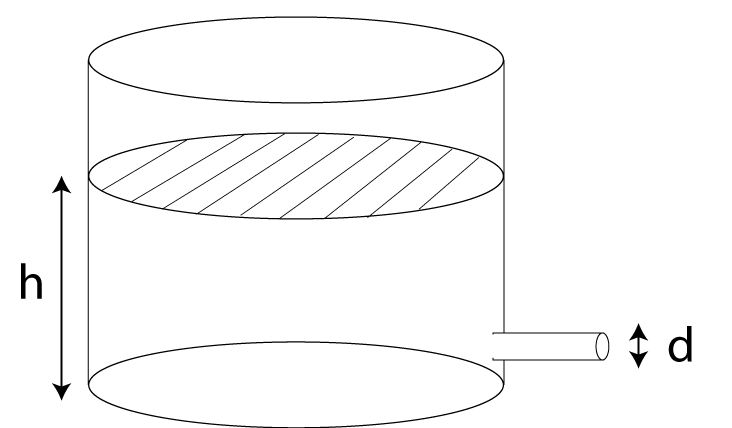
\includegraphics[width=0.45\textwidth]{figs/problema02.png}
	\end{figure}

	\startsolution

	\section*{Inciso (a)}
	Sabemos que la ecuación de Cauchy es

	\begin{equation*}
		\nabla \cdot{\bm{\sigma}} + \rho \vect{f} = \rho \mdv{\vect{v}}{t}.
	\end{equation*}

	Por la \zcref{eq:mdv-result-p1} y las hipótesis, la expresión anterior se ve como:

	\begin{equation*}
		-\nabla{p} - \rho \nabla{\phi} = \rho \Biggl(\pdv{\vect{v}}{t} + \nabla{\Bigl(\dfrac{v^{2}}{2}\Bigr)} -
		\cprod{\vect{v}}{( \cprod{\nabla}{\vect{v}} )}\Biggr),
	\end{equation*}

	y como el flujo es estacionario,

	\begin{equation}
		-\nabla{p} - \rho \nabla{\phi} = \rho \Biggl(\nabla{\Bigl(\dfrac{v^{2}}{2}\Bigr)} -
		\cprod{\vect{v}}{( \cprod{\nabla}{\vect{v}} )}\Biggr).
		\label{eq:cauchy-p4-dm}
	\end{equation}

	Calculando \(\dotprod{\vect{v}}{(\cdots)}\),

	\begin{equation*}
		-\dfrac{1}{\rho}\dotprod{\vect{v}}{\nabla{p}} - \dotprod{\vect{v}}{\nabla{\phi}} =
		\dotprod{\vect{v}}{\nabla{\Bigl(\dfrac{v^{2}}{2}\Bigr)}} -
		\dotprod{\vect{v}}{\Bigl(\cprod{\vect{v}}{( \cprod{\nabla}{\vect{v}} )}\Bigr)},
	\end{equation*}

	pero \(\dotprod{\vect{v}}{\Bigl(\cprod{\vect{v}}{( \cprod{\nabla}{\vect{v}} )}\Bigr)} = 0\).
	Así,

	\begin{equation}
		\dotprod{\vect{v}}{\nabla{\Bigl(\dfrac{v^{2}}{2} + \phi\Bigr)}} + \dfrac{1}{\rho}
		\dotprod{\vect{v}}{\nabla{p}} = 0.
		\label{eq:cauchy-second-simplification}
	\end{equation}

	Escribiendo el primer término como una divergencia,

	\begin{equation*}
		\nabla \cdot{\vect{v}\Bigl(\dfrac{v^{2}}{2} + \phi\Bigr)} =
		\Bigl(\dfrac{v^{2}}{2} + \phi\Bigr)(\nabla \cdot{\vect{v}}) +
		\dotprod{\vect{v}}{\nabla{\Bigl(\dfrac{v^{2}}{2} + \phi\Bigr)}},
	\end{equation*}

	pero \(\nabla \cdot{\vect{v}} = 0\) por ser incompresible, i.e.

	\begin{equation*}
		\nabla \cdot{\vect{v}\Bigl(\dfrac{v^{2}}{2} + \phi\Bigr)} =
		\dotprod{\vect{v}}{\nabla{\Bigl(\dfrac{v^{2}}{2} + \phi\Bigr)}},
	\end{equation*}

	Entonces, la \zcref{eq:cauchy-second-simplification} queda como:

	\begin{empheq}[box = \mainresult]{equation*}
		\nabla \cdot{\Bigl(\vect{v} \Bigl(\dfrac{v^{2}}{2} + \phi\Bigr)\Bigr)} +
		\dfrac{1}{\rho} \dotprod{\vect{v}}{\nabla{p}} = 0.
	\end{empheq}

	\section*{Inciso (b)}

	Como el flujo es irrotacional, la \zcref{eq:cauchy-p4-dm}se ve como:

	\begin{equation*}
		-\dfrac{1}{\rho}\nabla{p} - \nabla{\phi} = \nabla{\Bigl(\dfrac{v^{2}}{2}\Bigr)}.
	\end{equation*}

	Por lo tanto,

	\begin{empheq}[box = \mainresult]{equation*}
		\nabla{\Bigl(\dfrac{v^{2}}{2} + \phi\Bigr)} + \dfrac{1}{\rho}\nabla{p} = 0.
	\end{empheq}

	\section*{Inciso (c)}

	Del resultado anterior tenemos que

	\begin{align*}
		nabla{\Bigl(\dfrac{v^{2}}{2} + \phi + \dfrac{1}{\rho}p\Bigr)} & = 0,          \\
		\dfrac{v^{2}}{2} + \phi + \dfrac{1}{\rho}p                    & = \text{cte.}
	\end{align*}

	Es decir, para nuestro problema en particular tenemos

	\begin{equation*}
		\dfrac{v_{D}^{2}}{2} + \phi + \dfrac{1}{\rho}p_{D} = \dfrac{v_{d}^{2}}{2} + \phi + \dfrac{1}{\rho}p_{d},
	\end{equation*}

	donde \(\phi = gz\) pues la única fuerza de cuerpo que actúa sobre el fluido es la
	de la gravedad. Ahora, si colocamos nuestro sistema de referencia en \(z = 0\),
	tenemos que \(z_{d} = 0\) y \(z_{D} = h\). Así,

	\begin{equation*}
		\dfrac{v_{D}^{2}}{2} + gh + \dfrac{1}{\rho}p_{D} = \dfrac{v_{d}^{2}}{2} + \dfrac{1}{\rho}p_{d}.
	\end{equation*}

	Por otro lado, la presión \(p_{D} = p_{d} = p_{\text{atm}}\), entonces

	\begin{align}
		\dfrac{v_{D}^{2}}{2} + gh & = \dfrac{v_{d}^{2}}{2},\nonumber              \\
		v_{d}^{2}                 & = v_{D}^{2} + 2gh.\label{eq:velocidad-salida}
	\end{align}

	Y como to el fluido que baja del depósito sale por la boquilla,

	\begin{align*}
		v_{D}D \odif{t} = v_{d}d \odif{t}, \\
		v_{D} & = \dfrac{d}{D}v_{d}.
	\end{align*}

	Sustituyendo en la \zcref{eq:velocidad-salida},

	\begin{equation*}
		v_{d}^{2} = \dfrac{d^{2}}{D^{2}}v_{d}^{2} + 2gh,
	\end{equation*}

	pero \(\tfrac{d^{2}}{D^{2}} \sim 0\), ya que \(D^{2} \ggg d^{2}\). Por lo que
	la velocidad de salida es

	\begin{align*}
		v_{d}^{2}         & = 2gh,         \\
		\Aboxedmain{v_{d} & = \sqrt{2gh}.}
	\end{align*}

	Finalmente, para obtener el gasto volumétrico usamos que

	\begin{equation*}
		Q = Av.
	\end{equation*}

	Así,

	\begin{align*}
		Q             & = \Biggl(\pi \Bigl(\dfrac{d}{2}\Bigr)^{2}\Biggr)v_{d}, \\
		\Aboxedmain{Q & = \dfrac{\pi d^{2} v_{d}}{4}.}
	\end{align*}
\end{problema}
\end{document}
